\chapter{Model Architecture and Mathematical Formulation}
\label{ch:methodology}

\section{Overview of the Actor--Critic Architecture}
The portfolio management policy is trained using Proximal Policy Optimisation (PPO) \citep{schulman2017proximal} formulated within an Actor--Critic framework. The system architecture decouples temporal representation learning, continuous allocation policy parameterisation on the simplex manifold, and state-value baseline estimation:
\begin{enumerate}
    \item An \textbf{Encoder} processes the state observation to generate a compact 512-dimensional latent representation $\mathbf{h}_t \in \mathbb{R}^{512}$.
    \item An \textbf{Actor head} maps $\mathbf{h}_t$ to the parameters of a multivariate Dirichlet distribution that outputs portfolio allocations across $M = 11$ assets (10 equities plus cash).
    \item A \textbf{Critic head} maps $\mathbf{h}_t$ to a scalar baseline estimate $V_\phi(\mathbf{s}_t) \in \mathbb{R}$ approximating the expected cumulative discounted future reward.
\end{enumerate}

Figure~\ref{fig:architecture} illustrates the end-to-end information flow, and Figure~\ref{fig:pipeline} portrays the rollout interaction and PPO optimization pipeline.

\begin{figure}[htbp]
\centering
\begin{minipage}{0.49\textwidth}
\centering
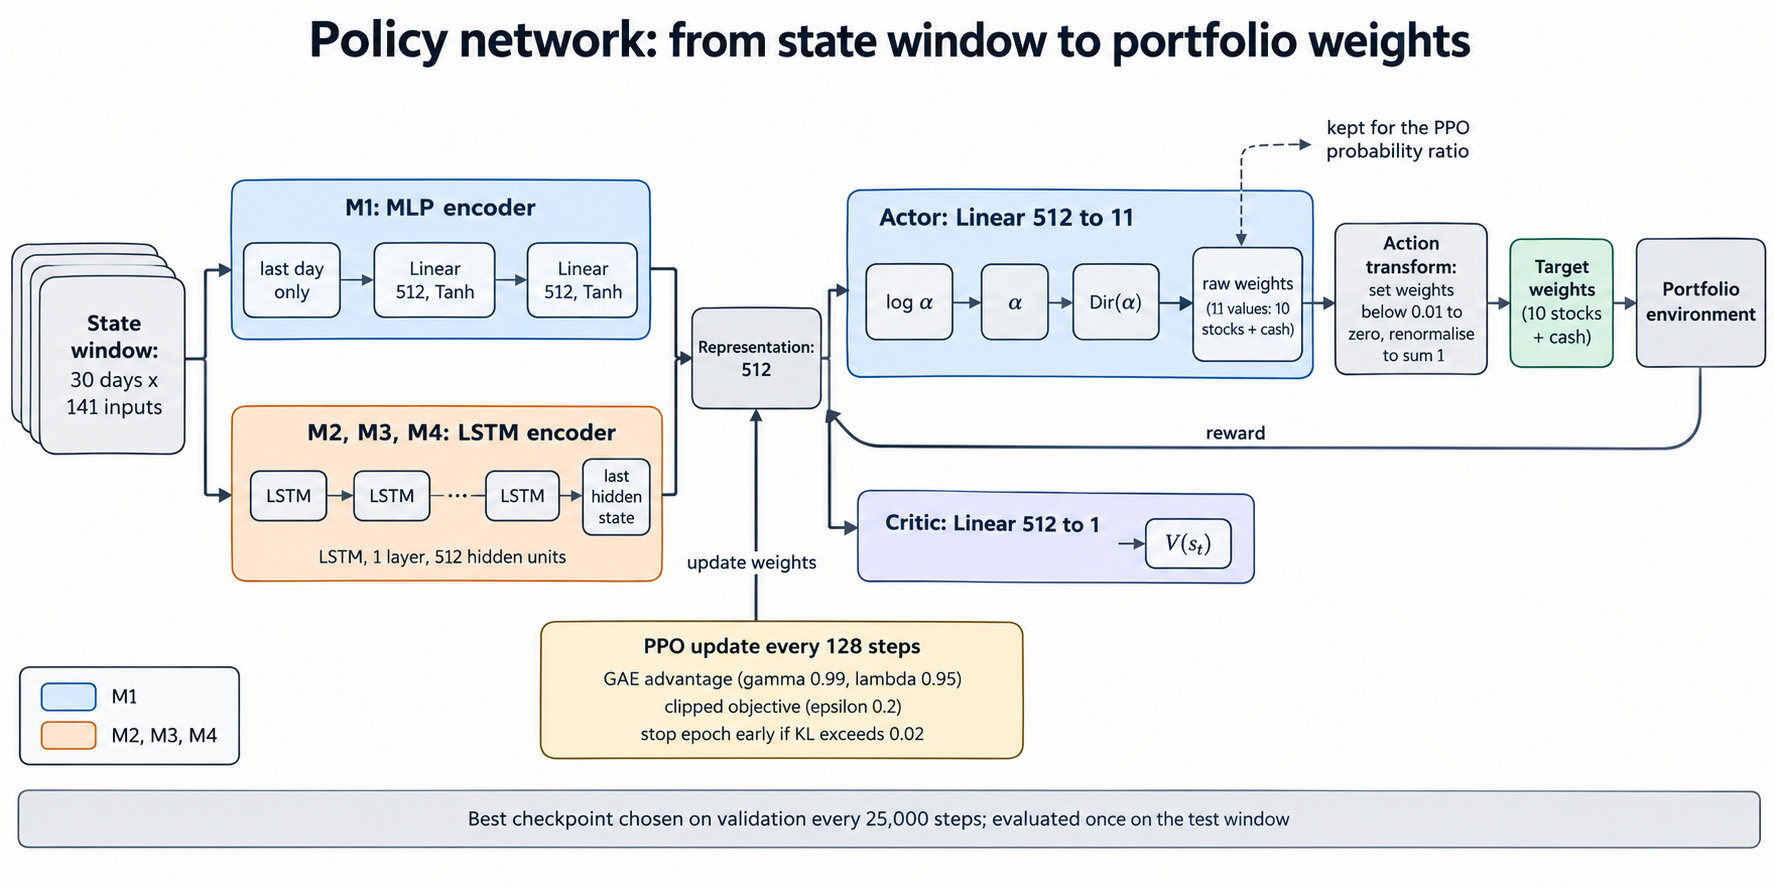
\includegraphics[width=\textwidth]{architecture.png}
\caption{Policy architecture from state to portfolio weights.}
\label{fig:architecture}
\end{minipage}\hfill
\begin{minipage}{0.49\textwidth}
\centering
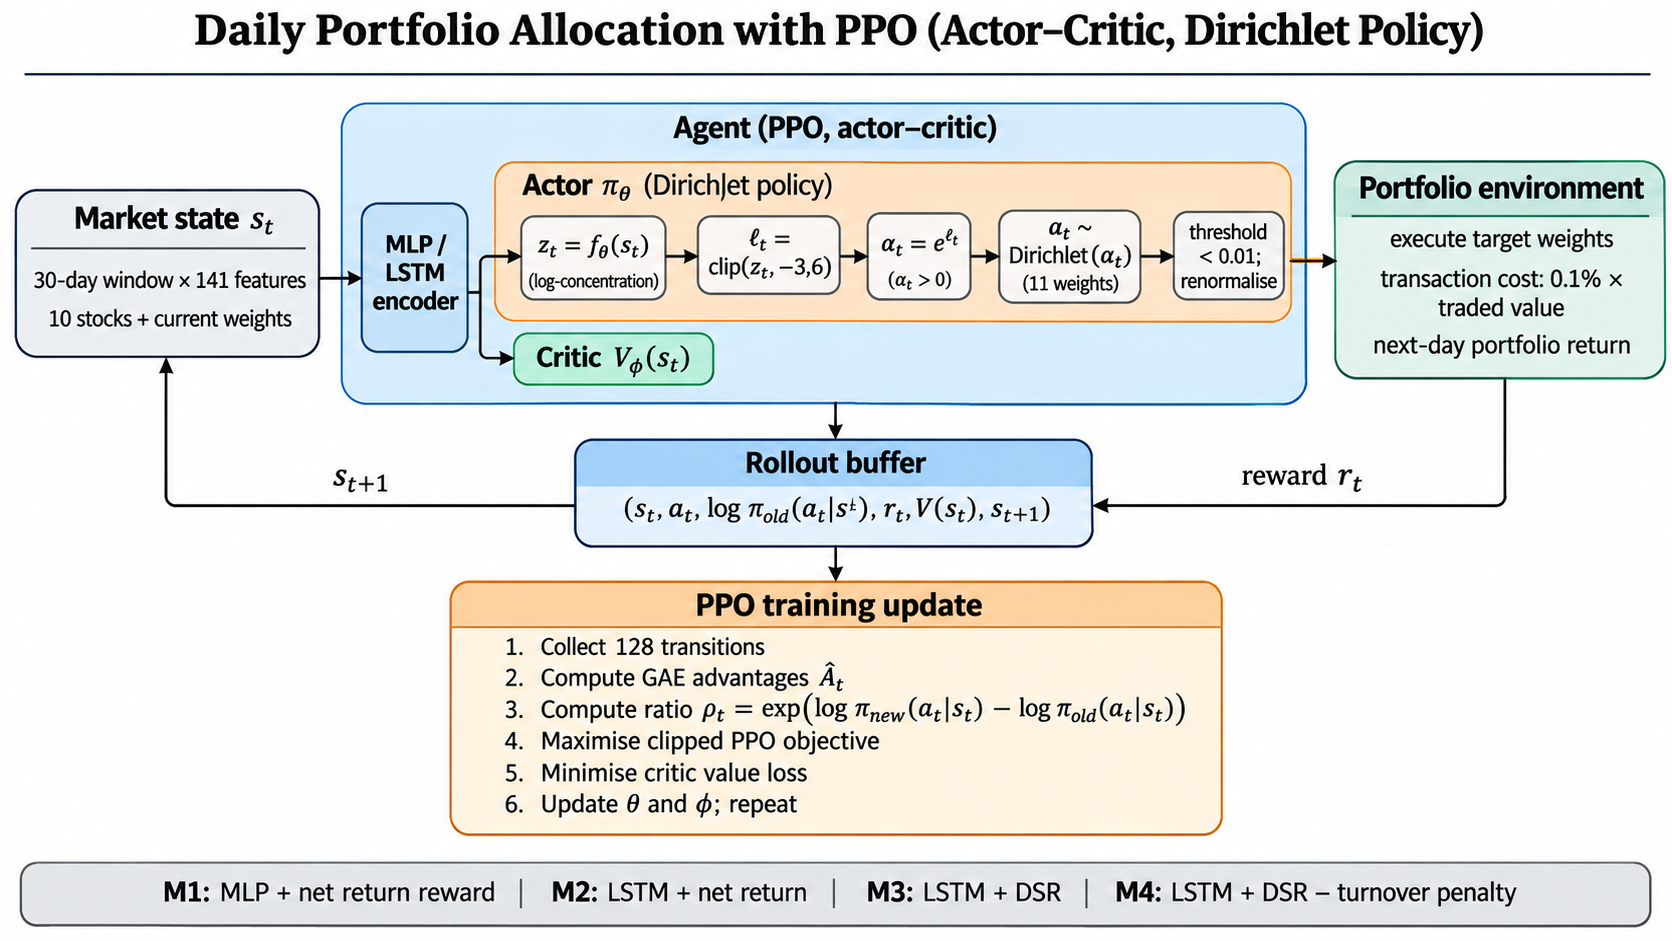
\includegraphics[width=\textwidth]{pipeline.png}
\caption{PPO Dirichlet allocation and environment loop.}
\label{fig:pipeline}
\end{minipage}
\end{figure}

\section{State Encoders: MLP versus Recurrent LSTM}
To rigorously evaluate the utility of temporal memory, two alternative encoder backbones are examined:

\subsection{Multi-Layer Perceptron (MLP) Encoder (Model M1)}
The feedforward MLP baseline observes solely the instantaneous observation vector at day $t$, $\mathbf{x}_t = \mathbf{s}_t \in \mathbb{R}^{141}$, discarding multi-period historical trajectories. The representation $\mathbf{h}_t$ is computed via two fully-connected layers with Tanh activations:
\begin{equation}
\mathbf{h}_t = \tanh\left( \mathbf{W}_2 \tanh\left( \mathbf{W}_1 \mathbf{x}_t + \mathbf{b}_1 \right) + \mathbf{b}_2 \right),
\end{equation}
where $\mathbf{W}_1 \in \mathbb{R}^{512 \times 141}$ and $\mathbf{W}_2 \in \mathbb{R}^{512 \times 512}$.

\subsection{Recurrent LSTM Encoder (Models M2--M4)}
To capture sequential price momentum and multi-period dependencies, Models M2, M3, and M4 pass the sliding history window $\mathbf{F}_t = [\mathbf{s}_{t-W+1}, \dots, \mathbf{s}_t] \in \mathbb{R}^{W \times 141}$ ($W = 30$) through a recurrent Long Short-Term Memory (LSTM) network:
\begin{equation}
(\mathbf{h}_t, \mathbf{c}_t) = \text{LSTM}(\mathbf{F}_t),
\end{equation}
with hidden representation size $H = 512$, following the empirical findings of \citet{zou2023novel}. The LSTM is trained end-to-end with the policy and value networks; rather than serving as an explicit price forecaster, $\mathbf{h}_t$ serves as a learned temporal belief state for sequential allocation.

\section{Continuous Dirichlet Policy on the Simplex}
\label{sec:dirichlet_policy}
A fundamental challenge in continuous portfolio control is ensuring that allocated asset weights satisfy the portfolio simplex constraints:
\begin{equation}
w_{i,t}^{\text{target}} \ge 0, \quad w_{\text{cash},t}^{\text{target}} \ge 0, \quad \sum_{i=1}^{N} w_{i,t}^{\text{target}} + w_{\text{cash},t}^{\text{target}} = 1.
\end{equation}
Following \citet{yang2022selective}, the policy is parameterised using a multivariate Dirichlet distribution, which natively defines a probability measure directly over the open unit simplex without requiring arbitrary heuristic projections.

\subsection{Actor Mapping to Dirichlet Parameters}
The actor network maps the latent representation $\mathbf{h}_t$ to an unconstrained linear vector $\mathbf{z}_t \in \mathbb{R}^{N+1}$:
\begin{equation}
\mathbf{z}_t = \mathbf{W}_a \mathbf{h}_t + \mathbf{b}_a, \quad \mathbf{W}_a \in \mathbb{R}^{(N+1) \times 512}, \; \mathbf{b}_a \in \mathbb{R}^{N+1}.
\end{equation}
To ensure numerical stability during gradient backpropagation, the outputs are clamped to a safe log-concentration range and exponentiated to yield strictly positive Dirichlet concentration parameters $\boldsymbol{\alpha}_t \in \mathbb{R}_{>0}^{N+1}$:
\begin{align}
\boldsymbol{\ell}_t &= \text{clip}\left( \mathbf{z}_t, -3.0, 6.0 \right), \\
\alpha_{i,t} &= \exp\left( \ell_{i,t} \right) \in \left[ e^{-3}, e^6 \right] \approx [0.0498, 403.43].
\end{align}
Clamping prevents underflow (which leads to degenerate distributions concentrated at vertices) and overflow (which causes numerical instability in the Gamma function derivative).

\subsection{Action Sampling and Expected Allocation}
The continuous action $\mathbf{a}_t \in \Delta^N$ is sampled from the Dirichlet probability density:
\begin{equation}
\label{eq:dirichlet_pdf}
\pi_\theta(\mathbf{a}_t \mid \mathbf{h}_t) = \frac{\Gamma\left( \sum_{i=1}^{N+1} \alpha_{i,t} \right)}{\prod_{i=1}^{N+1} \Gamma(\alpha_{i,t})} \prod_{i=1}^{N+1} a_{i,t}^{\alpha_{i,t} - 1},
\end{equation}
where $\Gamma(z)$ is the standard Gamma function. Sampling is performed via normalized independent Gamma variates: $g_{i,t} \sim \text{Gamma}(\alpha_{i,t}, 1)$ with $a_{i,t} = g_{i,t} / \sum_j g_{j,t}$. The expected portfolio allocation is:
\begin{equation}
\mathbb{E}\left[ a_{i,t} \right] = \frac{\alpha_{i,t}}{\sum_{j=1}^{N+1} \alpha_{j,t}}.
\end{equation}
During deterministic out-of-sample evaluation, the policy executes this expected allocation directly.

\subsection{Sparsity Thresholding and Renormalisation}
Because a Dirichlet distribution with positive parameters assigns non-zero mass across all assets, raw samples can contain minuscule allocations (e.g., $0.05\%$) that induce unneeded rebalancing fees. A threshold $\tau = 0.01$ (1\%) is applied identically across all models:
\begin{equation}
\label{eq:thresholding}
\tilde{w}_{i,t} = 
\begin{cases}
a_{i,t}, & \text{if } a_{i,t} \ge \tau, \\
0, & \text{if } a_{i,t} < \tau,
\end{cases}
\qquad
w_{i,t}^{\text{target}} = \frac{\tilde{w}_{i,t}}{\sum_{j=1}^{N+1} \tilde{w}_{j,t}}.
\end{equation}
This operation liquidates tiny positions and renormalises the surviving allocations to sum strictly to one.

\section{Portfolio Dynamics and Transaction Cost Accounting}
Let $\mathbf{w}_t^{\text{cur}} \in \Delta^N$ denote the portfolio weights immediately preceding rebalancing at day $t$. The required reallocation across the risky equities is $\Delta w_{i,t} = w_{i,t}^{\text{target}} - w_{i,t}^{\text{cur}}$.

Reallocating between cash and risky assets incurs a proportional transaction fee $c_{\text{trans}} = 0.001$ ($10\text{ bps}$):
\begin{equation}
C_t = c_{\text{trans}} V_{t-1} \sum_{i=1}^N \left| \Delta w_{i,t} \right|.
\end{equation}
End-of-day portfolio wealth $V_t$ evolves according to:
\begin{equation}
V_t = (V_{t-1} - C_t) \left[ \sum_{i=1}^N w_{i,t}^{\text{target}} (1 + R_{i,t}) + w_{\text{cash},t}^{\text{target}} \right],
\end{equation}
where $R_{i,t} = \frac{C_{i,t}}{C_{i,t-1}} - 1$ is the simple price return. The net portfolio return used throughout the framework is:
\begin{equation}
R_{\text{net},t} = \frac{V_t - V_{t-1}}{V_{t-1}}.
\end{equation}

\section{Model Reward Formulations (M1 to M4)}
The reward signal $r_t$ emitted to the agent constitutes the core ablation dimension:
\begin{enumerate}
    \item \textbf{Models M1 and M2 (Net Return Reward):}
    \begin{equation}
    r_t = R_{\text{net},t}.
    \end{equation}

    \item \textbf{Model M3 (Differential Sharpe Ratio):}
    Following \citet{millea2021deep}, an online recursive Differential Sharpe Ratio (DSR) is computed without requiring batch return histories. Moving estimates of the first and second return moments ($A_t \approx \mathbb{E}[R]$ and $B_t \approx \mathbb{E}[R^2]$) update exponentially with adaptation rate $\eta = 0.01$:
    \begin{align}
    A_t &= A_{t-1} + \eta (R_{\text{net},t} - A_{t-1}), \\
    B_t &= B_{t-1} + \eta (R_{\text{net},t}^2 - B_{t-1}).
    \end{align}
    With moment changes $\Delta A_t = A_t - A_{t-1}$ and $\Delta B_t = B_t - B_{t-1}$, the DSR reward is:
    \begin{equation}
    D_t = \frac{B_{t-1} \Delta A_t - \frac{1}{2} A_{t-1} \Delta B_t}{\left( B_{t-1} - A_{t-1}^2 + \varepsilon_{\text{DSR}} \right)^{3/2}},
    \end{equation}
    where $\varepsilon_{\text{DSR}} = 10^{-8}$ prevents numerical division by zero. For Model M3, $r_t = D_t$.

    \item \textbf{Model M4 (DSR with Squared Turnover Penalty):}
    To discourage excessive daily weight churn, an explicit quadratic turnover penalty is subtracted from the DSR reward:
    \begin{equation}
    r_t = D_t - \lambda_{\text{turn}} \sum_{i=1}^N \left( w_{i,t}^{\text{target}} - w_{i,t}^{\text{cur}} \right)^2,
    \end{equation}
    with $\lambda_{\text{turn}} = 0.1$ selected via validation tuning.
\end{enumerate}

\section{PPO Policy Optimisation}
During environment interaction, the agent collects transitions and stores the raw sampled continuous action $\mathbf{a}_t$ along with its log-likelihood under old parameters $\theta_{\text{old}}$:
\begin{equation}
\log \pi_{\theta_{\text{old}}}(\mathbf{a}_t \mid \mathbf{h}_t) = \ln \Gamma\left( \sum_{i=1}^{N+1} \alpha_{i,t} \right) - \sum_{i=1}^{N+1} \ln \Gamma(\alpha_{i,t}) + \sum_{i=1}^{N+1} (\alpha_{i,t} - 1) \ln a_{i,t}.
\end{equation}

Generalized Advantage Estimation (GAE) computes advantages $\hat{A}_t$ using temporal-difference residuals $\delta_t = \tilde{r}_t + \gamma V_\phi(\mathbf{s}_{t+1}) - V_\phi(\mathbf{s}_t)$ with discount $\gamma = 0.99$ and trace decay $\lambda_{\text{GAE}} = 0.95$:
\begin{equation}
\hat{A}_t = \sum_{l=0}^\infty (\gamma \lambda_{\text{GAE}})^l \delta_{t+l}.
\end{equation}

During mini-batch optimisation, the probability ratio is evaluated for the identical raw action $\mathbf{a}_t$:
\begin{equation}
\rho_t(\theta) = \frac{\pi_\theta(\mathbf{a}_t \mid \mathbf{h}_t)}{\pi_{\theta_{\text{old}}}(\mathbf{a}_t \mid \mathbf{h}_t)} = \exp\left( \log \pi_\theta(\mathbf{a}_t \mid \mathbf{h}_t) - \log \pi_{\theta_{\text{old}}}(\mathbf{a}_t \mid \mathbf{h}_t) \right).
\end{equation}
The policy parameters $\theta$ and critic parameters $\phi$ are updated by minimising the joint multi-task loss \citep{schulman2017proximal}:
\begin{equation}
\mathcal{L}(\theta, \phi) = -\hat{\mathbb{E}}_t \left[ \min\left( \rho_t(\theta) \hat{A}_t, \; \text{clip}(\rho_t(\theta), 1 - \epsilon, 1 + \epsilon) \hat{A}_t \right) \right] + c_1 \hat{\mathbb{E}}_t \left[ (V_\phi(\mathbf{s}_t) - \hat{V}_t^{\text{target}})^2 \right] - c_2 \hat{\mathbb{E}}_t [\mathcal{H}(\pi_\theta)],
\end{equation}
with clipping range $\epsilon = 0.2$, critic weight $c_1 = 0.5$, and entropy bonus $c_2 = 0.01$.

\begin{figure}[htbp]
\centering
\begin{minipage}{0.96\textwidth}
\hrule \vspace{2pt} \hrule \vspace{4pt}
\noindent\textbf{Algorithm 1: PPO Daily Portfolio Allocation with Dirichlet Policy}
\vspace{4pt} \hrule \vspace{6pt}
\footnotesize
\noindent\textbf{Input:} Market series $\mathbf{X}$, returns $\mathbf{R}$, cost $c_{\text{trans}}$, threshold $\tau$, penalty $\lambda_{\text{turn}}$, PPO parameters $\gamma, \lambda_{\text{GAE}}, \epsilon, \eta_{\text{LR}}$.\\
\textbf{Initialisation:} Actor $\theta$, Critic $\phi$, reward normaliser $\mathcal{N}$, initial weights $\mathbf{w}_0^{\text{cur}} \gets [0, \dots, 0, 1]^\top$ (cash), DSR moments $A \gets 0, B \gets 0$.
\vspace{4pt}
\begin{enumerate}
    \item \textbf{for} $\text{iteration} = 1, 2, \dots$ until $T_{\text{total}} = 300,000$ steps \textbf{do}
    \item \quad Reset rollout buffer $\mathcal{B} \gets \emptyset$.
    \item \quad \textbf{for} $t = 1$ to $T_{\text{rollout}} = 128$ \textbf{do}
    \item \qquad Compute representation $\mathbf{h}_t \gets \text{Encoder}(\mathbf{s}_t)$ (MLP for M1; LSTM for M2--M4).
    \item \qquad Compute concentrations $\boldsymbol{\ell}_t \gets \text{clip}(\mathbf{W}_a \mathbf{h}_t + \mathbf{b}_a, -3, 6)$ and $\boldsymbol{\alpha}_t \gets \exp(\boldsymbol{\ell}_t)$.
    \item \qquad Sample raw action variates $g_i \sim \text{Gamma}(\alpha_{i,t}, 1)$, set $\mathbf{a}_t \gets \mathbf{g} / \sum_i g_i$.
    \item \qquad Evaluate old log-likelihood $lp_t \gets \log \pi_\theta(\mathbf{a}_t \mid \mathbf{h}_t)$ and value $V_t \gets V_\phi(\mathbf{h}_t)$.
    \item \qquad Apply threshold $\tau = 0.01$: $\tilde{w}_i \gets a_{i,t} \cdot \mathbf{1}_{a_{i,t} \ge \tau}$, set $\mathbf{w}_t^{\text{target}} \gets \tilde{\mathbf{w}} / \sum_j \tilde{w}_j$.
    \item \qquad Execute trade: compute $\text{Turnover}_t$, cost $C_t$, net return $R_{\text{net},t}$, new wealth $V_t$.
    \item \qquad Compute model reward $r_t$ (Net return for M1/M2; DSR for M3; DSR $-\lambda_{\text{turn}} \sum (\Delta w_i)^2$ for M4).
    \item \qquad Store transition $(\mathbf{s}_t, \mathbf{a}_t, lp_t, V_t, r_t)$ in buffer $\mathcal{B}$.
    \item \quad \textbf{end for}
    \item \quad Compute GAE advantages $\hat{A}_t$ and return targets $\hat{V}_t^{\text{target}}$.
    \item \quad \textbf{for} $\text{epoch} = 1$ to $K = 10$ \textbf{do}
    \item \qquad \textbf{for} each minibatch of size $B = 64$ \textbf{do}
    \item \qquad\quad Evaluate current log-likelihoods $\log \pi_\theta(\mathbf{a}_i \mid \mathbf{h}_i)$ and values $V_\phi(\mathbf{h}_i)$.
    \item \qquad\quad Compute probability ratio $\rho_i(\theta) \gets \exp(\log \pi_\theta - lp_i)$ and multi-task loss $\mathcal{L}(\theta, \phi)$.
    \item \qquad\quad Update $(\theta, \phi)$ via Adam optimiser ($\eta_{\text{LR}} = 10^{-4}$) with gradient clipping $0.5$.
    \item \qquad \textbf{end for}
    \item \quad \textbf{end for}
    \item \textbf{end for}
\end{enumerate}
\vspace{4pt} \hrule
\end{minipage}
\caption{Complete training and policy update algorithm for PPO portfolio allocation.}
\label{alg:ppo_portfolio}
\end{figure}
